\section{Constellation Orbital Parameters}
\definecolor{blue}{rgb}{0.2,0.5,0.8}

\begin{minipage}{0.5\textwidth}
\begin{tabular}{|l|c|}
	\hline
	Number of satellites & 189 \\ \hline
	Number of Planes & 9 \\ \hline
	Num. Satellites/Plane & 21 \\ \hline
	Height of the orbits (km) & 542 \\ \hline
	Constellation Type & Walker-Delta \\ \hline
	Planes Inclination & 72 \\ \hline
	Orbital Periods (min) & 95.48 \\ \hline
	Minimum Elevation (deg) & 20 \\ \hline
	Mean Pass time (min) & 4.28 \\ \hline
\end{tabular}
\end{minipage} \hfill
\begin{minipage}{0.45\textwidth}
\begin{figure}[H]
	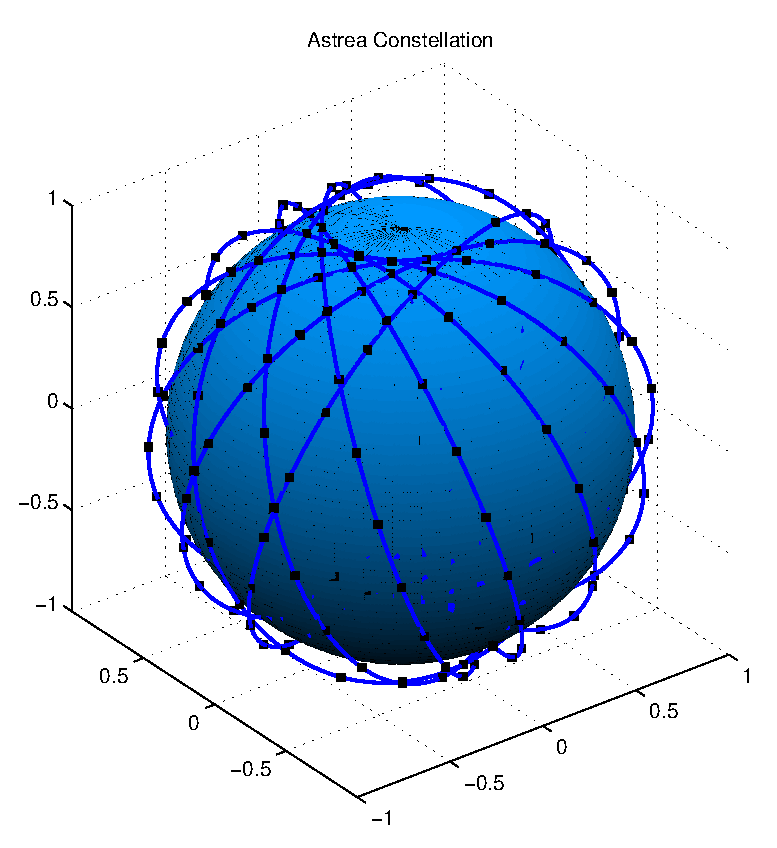
\includegraphics[scale=0.6]{ConstellationSphere}
	\caption{Spherical Distribution of the Constellation}	
\end{figure}
\end{minipage}

\begin{figure}[h]
	\centering  
	\includegraphics[scale=0.6]{ConstellationPlain}
	\caption{Ground Track Example}	
\end{figure}

\newpage

\paragraph{Planes distribution of the Astrea Constellation \\}
The AstreaSATs are distributed in 9 plains. Even though there is symmetry inside each plane, the plains are not distributed equally in space. Their Right Arguments of the Ascendent Node are splitted regularly in a sector of 225 degrees, giving shape to the table and figures below:

\begin{figure}[h]
	\centering  
	\includegraphics[scale=0.8]{PlanesDistrib}
	\caption{Planes distribution representation. Left: From a top view, the pattern that the orbital planes generate. Right: The planes normal vectors in the fan they create.}	
\end{figure}

\centering
\begin{tabular}{|c|c|}
\hline
\textbf{Plane} & \textbf{RAAN(º)} \\ \hline 
1 & 0 \\ \hline
2 & 28.125 \\ \hline
3 & 56.25 \\ \hline
4 & 84.375 \\ \hline
5 & 112.5 \\ \hline
6 & 140.625 \\ \hline
7 & 168.75 \\ \hline
8 & 196.875 \\ \hline
9 & 225 \\ \hline
\end{tabular}